\section{Results}

\begin{figure*}[!t]
    \centering
    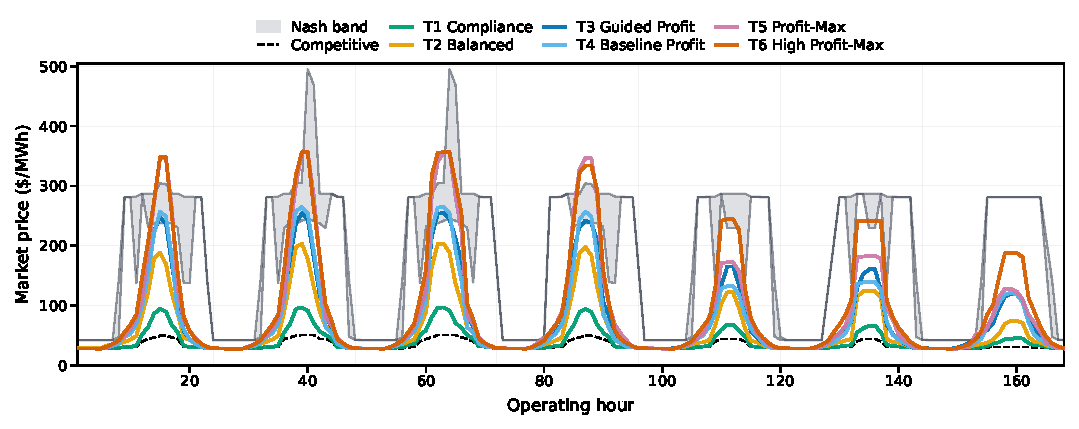
\includegraphics[
        width=0.90\textwidth,
        height=0.20\textheight,
        keepaspectratio
    ]{figures/figure_1_all_treatments_overlay_twocolumn}
    \caption{Hourly price trajectories by prompt treatment. Lines show treatment-average prices for all six prompt objectives; the dashed line shows the perfect competition benchmark and the shaded band shows the Nash benchmark range. More profit-oriented prompt treatments produce higher prices during peak and near-scarcity hours.}
    \label{fig:price_trajectories}
    \vspace{-0.6em}
\end{figure*}
% Table II: Treatment-level outcomes with vertically stacked confidence intervals
% Requires: \usepackage{booktabs}

\begin{table*}[t]
\centering
\caption{Treatment-Level Outcomes by Prompt Objective}
\label{tab:treatment_summary}
\scriptsize
\renewcommand{\arraystretch}{1.12}
\setlength{\tabcolsep}{3.6pt}
\begin{tabular}{@{}lrrrrr@{}}
\toprule
Treatment & Prompt $S_t$ & TARJ orient. & Mean markup & $\Delta P$ (\$/MWh) & $\Delta \Pi$ (\$M) \\
\midrule
T1 Compliance & $-0.134$ &
\begin{tabular}{@{}c@{}}$-0.011$\\{\scriptsize [$-0.015$, $-0.007$]}\end{tabular} &
\begin{tabular}{@{}c@{}}1.144\\{\scriptsize [1.129, 1.159]}\end{tabular} &
\begin{tabular}{@{}c@{}}6.87\\{\scriptsize [5.87, 7.90]}\end{tabular} &
\begin{tabular}{@{}c@{}}7.33\\{\scriptsize [6.31, 8.00]}\end{tabular} \\
\addlinespace[0.25em]
T2 Balanced & 0.009 &
\begin{tabular}{@{}c@{}}0.028\\{\scriptsize [0.024, 0.032]}\end{tabular} &
\begin{tabular}{@{}c@{}}1.591\\{\scriptsize [1.547, 1.632]}\end{tabular} &
\begin{tabular}{@{}c@{}}25.32\\{\scriptsize [21.98, 28.73]}\end{tabular} &
\begin{tabular}{@{}c@{}}26.77\\{\scriptsize [23.59, 29.72]}\end{tabular} \\
\addlinespace[0.25em]
T3 Guided Profit & 0.060 &
\begin{tabular}{@{}c@{}}0.057\\{\scriptsize [0.054, 0.060]}\end{tabular} &
\begin{tabular}{@{}c@{}}1.919\\{\scriptsize [1.848, 1.990]}\end{tabular} &
\begin{tabular}{@{}c@{}}40.67\\{\scriptsize [36.60, 44.89]}\end{tabular} &
\begin{tabular}{@{}c@{}}42.43\\{\scriptsize [38.12, 47.12]}\end{tabular} \\
\addlinespace[0.25em]
T4 Baseline Profit & 0.125 &
\begin{tabular}{@{}c@{}}0.066\\{\scriptsize [0.061, 0.070]}\end{tabular} &
\begin{tabular}{@{}c@{}}1.883\\{\scriptsize [1.769, 1.998]}\end{tabular} &
\begin{tabular}{@{}c@{}}38.26\\{\scriptsize [31.97, 44.57]}\end{tabular} &
\begin{tabular}{@{}c@{}}40.04\\{\scriptsize [28.20, 49.31]}\end{tabular} \\
\addlinespace[0.25em]
T5 Profit-Max & 0.132 &
\begin{tabular}{@{}c@{}}0.065\\{\scriptsize [0.061, 0.068]}\end{tabular} &
\begin{tabular}{@{}c@{}}2.382\\{\scriptsize [2.267, 2.523]}\end{tabular} &
\begin{tabular}{@{}c@{}}56.15\\{\scriptsize [49.11, 62.95]}\end{tabular} &
\begin{tabular}{@{}c@{}}58.85\\{\scriptsize [56.32, 61.41]}\end{tabular} \\
\addlinespace[0.25em]
T6 High Profit-Max & 0.147 &
\begin{tabular}{@{}c@{}}0.067\\{\scriptsize [0.064, 0.070]}\end{tabular} &
\begin{tabular}{@{}c@{}}2.700\\{\scriptsize [2.593, 2.809]}\end{tabular} &
\begin{tabular}{@{}c@{}}65.30\\{\scriptsize [60.12, 70.63]}\end{tabular} &
\begin{tabular}{@{}c@{}}68.15\\{\scriptsize [61.41, 74.89]}\end{tabular} \\
\bottomrule
\end{tabular}

\vspace{1.0em}
\begin{minipage}{0.90\textwidth}
\footnotesize
\emph{Note:} Bracketed values report 95\% bootstrap intervals. $S_t$ is the SBERT prompt profit-minus-compliance orientation. $\Delta P$ is average price increase relative to the competitive benchmark, and $\Delta \Pi$ is firm profit gain. Price, markup, and TARJ intervals resample seed--day blocks within treatment; firm-profit intervals resample seed-level treatment runs. TARJ orientation is post-treatment and is reported as behavioral alignment rather than a causal mechanism.
\end{minipage}
\vspace{-0.4em}
\end{table*} 

\subsection{Economic Benchmark Comparison}

We first compare LLM-agent market outcomes with the perfect competition and strategic Nash Equilibrium benchmarks. The perfect competition benchmark clears the same market using cost-based offers, so it provides the reference price path for measuring price impacts. The Nash benchmark provides a useful strategic reference because it represents equilibrium behavior under the same market environment and markup grid available to the LLM agents. Since some hours have multiple pure-strategy equilibria, we report an hourly Nash price band rather than a single price. The band is not evidence that the agents solved for equilibrium. Instead, it shows whether their bids move market outcomes away from the perfect competition benchmark and toward the strategically elevated prices that are feasible under model conditions.

Figure~\ref{fig:price_trajectories} shows that the prompt treatments produce visibly different price trajectories. As the profit orientation ($S_t$) of treatments increases, we observe more aggressive bidding behavior and higher market prices.  T1 Compliance remains closest to the perfect competition benchmark. Intermediate treatments raise prices during high-load hours, while the most profit-oriented treatments, especially T5 Profit-Max and T6 High Profit-Max, move prices closer to strategic pricing and the Nash band during peak and near-scarcity periods. This is consistent with the electricity-market intuition that strategic markups matter most when supply is tight and the marginal unit has greater price-setting influence.


\subsection{Treatment-Level Outcomes}

Table~\ref{tab:treatment_summary} summarizes the treatment-level semantic and market outcomes. As objectives become more profit-oriented, average price impacts generally increase: from $\$6.87$/MWh under T1 Compliance to $\$65.30$/MWh under T6 High Profit-Max. The ordering is not perfectly monotonic, since T3 has lower prompt orientation than T4 but a slightly higher average price impact. Nevertheless, there is a clear emerging pattern. Compliance-oriented prompting produces outcomes closest to the perfect competition benchmark, while increasingly profit-oriented prompting pushes prices upward toward the strategic price range indicated by the Nash band.

The markup and profit results show the same directional pattern. Mean markup increases from 1.144 under T1 to 2.700 under T6, and firm profit gain rises from \$7.33M to \$68.15M. These increases suggest that more aggressive profit-maximizing language pushes agents to submit higher markups and capture larger profits. However, this effect is bounded. In this case study, prices are limited by the finite markup grid, the underlying supply stack, demand conditions, and the availability of the backstop resource. The Nash band therefore provides a useful reference for interpreting the upper strategic range. It does not represent a hard cap on every possible non-equilibrium bid outcome, but it shows the elevated price region consistent with equilibrium play under the same model assumptions. The main result is that changing only the objective block of the prompt moves simulated bidding behavior from near-competitive outcomes toward this strategic benchmark range.


\subsection{Semantic Orientation, Prompt Selection, and Market Outcomes}

Figure~\ref{fig:semantic_orientation} relates semantic profit-minus-compliance orientation to market outcomes, showing whether the SBERT ordering used to characterize and select prompts is reflected in bidding behavior. Panels A and B use the SBERT orientation of the objective prompt, which is measured before simulation and represents the treatment's position along the compliance-profit axis. Panels C and D use the SBERT orientation of generated TARJ rationales, which are post-treatment text artifacts produced by the agents during the simulation. Prompt orientation therefore measures the intervention, while TARJ orientation measures agent-generated explanations for bidding behavior.
\begin{figure}[!t]
    \centering
    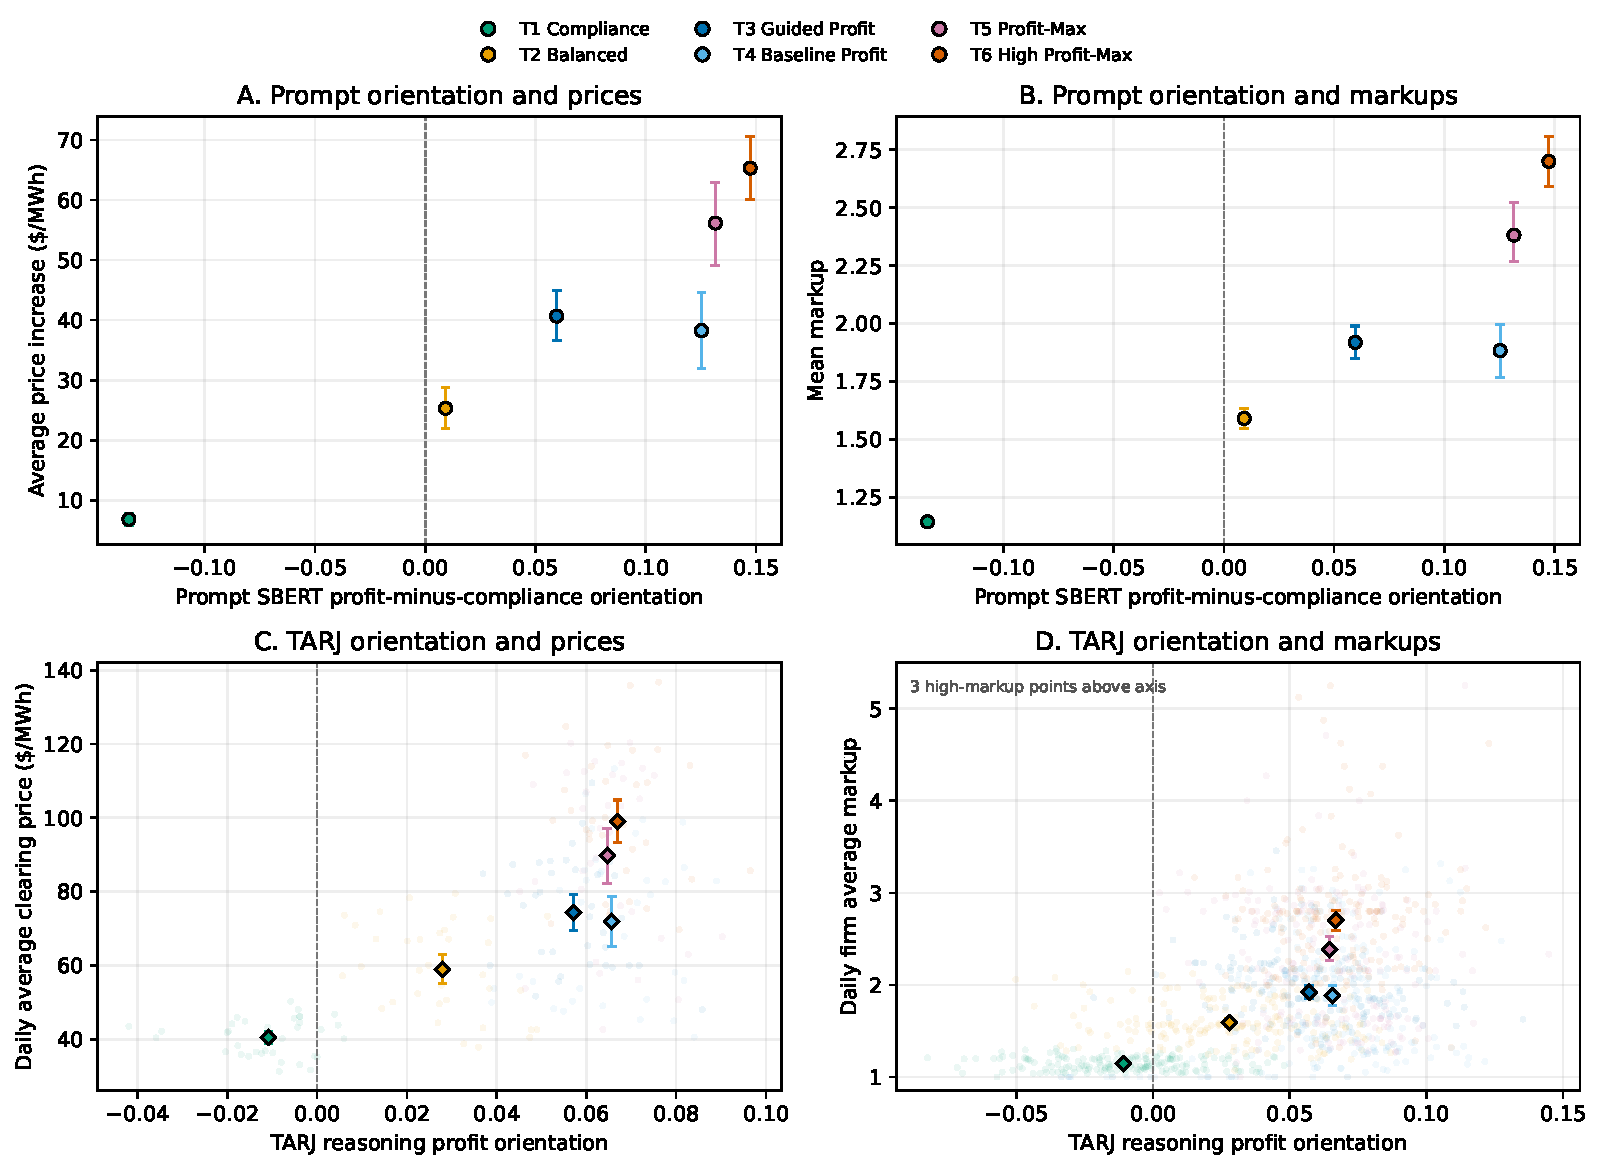
\includegraphics[
        width=0.99\columnwidth,
        height=0.55\textheight,
        keepaspectratio
    ]{figures/figure_2_semantic_orientation_main_no_spearman}
    \caption{Semantic orientation, prices, and bidding behavior. Panels A--B compare prompt orientation with average price increases and mean markups; Panels C--D compare TARJ orientation with daily prices and firm markups. Error bars report 95\% bootstrap intervals.}
    \label{fig:semantic_orientation}
    \vspace{-0.8em}
\end{figure}
The main statistical result is a treatment-level relationship between prompt orientation and market outcomes, estimated using \eqref{eq:dose_response}.

\begin{table}[!t]
\centering
\caption{SBERT Orientation Regression Coefficients}
\label{tab:dose_response_summary}
\scriptsize
\renewcommand{\arraystretch}{1.05}
\setlength{\tabcolsep}{2.8pt}
\begin{tabular}{@{}lcccc@{}}
\toprule
Outcome & $\hat{\beta}_{0.1}$ & 95\% CI & $R^2$ & $p$ \\
\midrule
$\Delta P$ (\$/MWh) & 18.17 & [7.85, 28.49] & 0.857 & 0.008 \\
Mean markup & 0.465 & [0.153, 0.778] & 0.810 & 0.014 \\
Firm profit (\$M) & 18.93 & [8.21, 29.65] & 0.857 & 0.008 \\
Consumer payments (\$M) & 19.02 & [8.35, 29.70] & 0.860 & 0.008 \\
Mean TARJ orientation & 0.029 & [0.021, 0.036] & 0.967 & $<0.001$ \\
\bottomrule
\end{tabular}

\vspace{0.25em}
\begin{minipage}{0.96\columnwidth}
\footnotesize
\emph{Note:} Estimates come from treatment-level regressions $\bar{Y}_t=\alpha+\beta S_t+\epsilon_t$, where $S_t$ is prompt SBERT profit-minus-compliance orientation. Coefficients are scaled to a 0.1 increase in prompt orientation. CIs use OLS standard errors across the six treatment means with four residual degrees of freedom.
\end{minipage}
\vspace{-0.8em}
\end{table}

As shown in Table~\ref{tab:dose_response_summary}, a 0.1 increase in prompt orientation is associated with an estimated $\$18.17$/MWh increase in average price impact relative to the perfect competition benchmark. The same pattern appears for bidding aggressiveness: a 0.1 increase in prompt orientation is associated with a 0.465 increase in mean markup. The table also shows positive associations with firm profit gains, consumer payment increases, and TARJ reasoning orientation. These relationships are also statistically strong within the six-treatment design, with the $R^2$ values in Table~\ref{tab:dose_response_summary} ranging from 0.810 to 0.967, and all reported $p$-values are below 0.05. Because the regressions use treatment-level means, we interpret these statistics as evidence of within-case alignment rather than as broad population-level inference.

A similar relationship also appears in distributional market outcomes. A 0.1 increase in prompt orientation is associated with an estimated $\$18.93$M increase in firm profit gain and a $\$19.02$M increase in consumer payments. Prompt orientation is also strongly associated with generated reasoning language. A 0.1 increase in prompt orientation is associated with a 0.029 increase in mean TARJ reasoning orientation. This is the expected direction under the proposed framework. Prompts that are semantically closer to profit maximization are intended to induce more aggressive bidding, higher market prices, and higher firm profits if the prompt intervention is functioning properly.

The TARJ-orientation panels (C and D) provide a secondary result. More profit-oriented generated reasoning accompanies higher prices and more aggressive markups, but this relationship is interpreted differently from the prompt-orientation relationship. TARJ text is generated after the prompt intervention, so it is treated as a way to analyze agent reasoning in addition to bidding behavior. This alignment is important because it suggests that the framework is not only detecting changes in bidding behavior, but also validating that prompt meaning, generated reasoning, and bidding posture are aligned.
